\section{Introduction}
\label{sec:intro}

A language model that automates a step in a program has to do more than produce a good answer. It has
to say how likely that answer is to be right, in a form that the program can act on: answer when the
probability is high, and abstain or hand the case to another model or a person when it is not. The rule
is only as good as the number it reads. A confidence is \emph{calibrated} when, among the cases to which
the model gives probability $p$, a fraction $p$ is correct~\citep{guo2017calibration}; a threshold
policy built on a miscalibrated confidence answers when it should not, or escalates cases it could have
settled.

% AUTO-GENERATED by build/gen_jev_market.py from literature/notes/jev_hf_268.tsv -- do not hand-edit.
\begin{table}[tp]
\centering\footnotesize
\renewcommand{\arraystretch}{1.18}
\caption{\textbf{Repositories returned by the Hugging Face model search for ``jev'', by application} (snapshot of
2026-09-27). \href{https://typesafe.ai/blog/introducing-system-one-models-and-jev}{Jev} is a hosted model from TypeSafe AI, released on 2026-09-15~\citep{almeida2026introducing},
that returns a probability for each declared option (a typed decision, Table~\ref{tab:definitions}). Of the 268
repositories the search returns, 76 only share the name (75 predate Jev) and 4
could not be verified (empty, without a card, or gated with no public card metadata); the remaining 188 are classified here from their
model cards and file lists (for a gated repository, from its public card metadata), with an application category taking
precedence over a language one. Downloads are over the last
30 days. 137 repositories contain newly trained weights; the 38 copies, ports and packages add
none (the 6 mirrors contain their source's weight files byte for byte). General-purpose models and the
copies of them account for 87\% of the 41,653 downloads in the table. A name search misses most decision models: of the
51 open systems with released weights on the Jev Decision Index (Table~\ref{tab:jev_decision_index}), it returns 4.}
\Description{A table with one row per application category of the repositories returned by the Hugging Face search for jev,
giving the number of repositories, their downloads over thirty days and linked example repositories. General-purpose typed-decision models are
the largest group, followed by research checkpoints and copies.}
\label{tab:jev_hf_ecosystem}
\begin{tabular}{@{}>{\raggedright\arraybackslash}p{0.24\textwidth}rr>{\raggedright\arraybackslash}p{0.45\textwidth}@{}}
\toprule
\textbf{Category} & \textbf{Repositories} & \textbf{Downloads} & \textbf{Examples} \\
\midrule
General-purpose typed-decision model & 55 & 19,655 & \href{https://huggingface.co/alibiserikbay/JevK5}{JevK5}, \href{https://huggingface.co/ZefanCai/Open-Jev-9B}{Open-Jev-9B}, \href{https://huggingface.co/com-kotobalabs/open-jev-deberta-v3-large}{open-jev-deberta}, \href{https://huggingface.co/lostargon/Tiny-Jev}{Tiny-Jev}, \href{https://huggingface.co/chaoliangUNSW/Jev-Style-0.8B-Decision-v3}{Jev-Style v3} \\
Research and ablation checkpoints & 45 & 212 & \href{https://huggingface.co/Praveenrajus/jevify-qwen3.5-4b-readout-coh}{jevify} (31-checkpoint readout series), \href{https://huggingface.co/JonesLin/next-jev-stage1-cot}{next-jev} (latent-workspace study), \href{https://huggingface.co/ryandcunha/mmbu-jev-qwen3-0.6b-closed}{mmbu-jev} (closed-set vs free-text) \\
Copy, port or package (no new training) & 38 & 18,640 & \href{https://huggingface.co/mradermacher/JEV-9B-GGUF}{JEV-9B-GGUF} (GGUF), \href{https://huggingface.co/Ruiruiz30/Jev-Omni-MLX-4bit}{Jev-Omni-MLX-4bit} (MLX), \href{https://huggingface.co/onnx-community/open-jev-deberta-v3-large-ONNX}{open-jev-deberta-ONNX} (ONNX), \href{https://huggingface.co/liodon-ai/JevK5-FP8}{JevK5-FP8} (FP8), \href{https://huggingface.co/junetask/Open-Jev-9B}{junetask/Open-Jev-9B} (a mirror) \\
No newly trained model (recipe, runtime, code or data) & 11 & 0 & \href{https://huggingface.co/NicolaiMTLassen/bonzi-8b-v1-jev}{bonzi} (recipes), \href{https://huggingface.co/Meanblock/JEV-CPU}{JEV-CPU} (code), \href{https://huggingface.co/SargeDev/jev-distill-corpus}{jev-distill-corpus} (dataset) \\
Agents, tools and safety & 10 & 1,005 & \href{https://huggingface.co/samatv256/mini-Jev}{mini-Jev} (tool routing), \href{https://huggingface.co/nicolasembleton/mini-jev-minicpm5-2b-shell-safety-phase1b-merged}{Mini-Jev shell-safety}, \href{https://huggingface.co/SargeDev/jev-gate-student-b}{Jev-Gate} (memory gating), \href{https://huggingface.co/atmaneayoub/jev-ar}{jev-ar} (Gulf-Arabic intent routing) \\
Domain application & 10 & 152 & \href{https://huggingface.co/Nebulaw1/jev-qwen3.5-4b-legal-lora}{jev-legal} (Chinese legal), \href{https://huggingface.co/mogita/jev-decider-qwen3-4b}{jev-decider} (bank transactions), \href{https://huggingface.co/guzus/jev-nyotti}{jev-nyotti} (BTC trading), \href{https://huggingface.co/wendellperbar/serigy-jev}{Serigy-Jev} (PT-BR fake news), \href{https://huggingface.co/sdmlai/nano-jev}{Nano-Jev} (RAG) \\
Language-specific & 7 & 1,010 & \href{https://huggingface.co/argos1111/modernbert-ja-310m-jev}{modernbert-ja-jev} (Japanese), \href{https://huggingface.co/wwydmanski/bielik-minitron-jev-v0.3}{bielik-minitron-jev} (Polish), \href{https://huggingface.co/nouton/jev-ru-4b-lora-v2}{Jev-RU} (Russian, Ukrainian, Belarusian) \\
Multimodal or vision & 5 & 594 & \href{https://huggingface.co/akhilaaa3/Jev-Omni}{Jev-Omni} (text, image, audio, video), \href{https://huggingface.co/SeanLiu/Jev-Vision}{Jev-Vision}, \href{https://huggingface.co/Fr0zencr4nE/jev-spatial}{Jev-Spatial} \\
Games and control & 5 & 156 & \href{https://huggingface.co/SUPER321/jevflash-doom-basic-0.6b}{JevFlash} (Doom), \href{https://huggingface.co/bzantium/gemma-3-270m-jev}{gemma-3-270m-jev} (ViZDoom), \href{https://huggingface.co/zwh20081/hoi4-jevai}{JevAI} (Hearts of Iron IV mod) \\
Embeddings trained on typed-decision questions & 2 & 229 & \href{https://huggingface.co/HIT-TMG/JevEmbed-KaLM-Embedding-V2.5}{JevEmbed-KaLM}, \href{https://huggingface.co/HIT-TMG/JevEmbed-Qwen3-Embedding-0.6B}{JevEmbed-Qwen3} \\
\midrule
\textbf{Total} & \textbf{188} & \textbf{41,653} & \\
\bottomrule
\end{tabular}
\end{table}

% AUTO-GENERATED by build/gen_jev_market.py from literature/notes/jev_decision_index_2026-09-27.json -- do not hand-edit.
\begin{table}[tp]
\centering\footnotesize
\setlength{\tabcolsep}{3.5pt}
\caption{\textbf{Jev and open decision models on the Jev Decision Index}: ranks 1 to 15 of the 68
systems on the \href{https://huggingface.co/spaces/multimodalart/jev-decision-index}{Jev Decision Index}~\citep{multimodalart2026jevdi} (release 0.2.1,
data of 2026-09-27). Skill is chance-normalised (0 to 100) over the same 38-benchmark
panel for every system, and unanswered requests count as wrong. ECE is measured on a one-in-6
sample of 32 benchmarks with a per-field right answer. The board reports point estimates
without uncertainty intervals. Base model and method are as recorded by the board: full fine-tune, a low-rank adapter (LoRA), a trained head or adapter over a frozen model, inference only (prompting or decoding over unchanged weights) or a hosted API. Names link to the
model's Hugging Face repository, or to its code where no weights are released. Jev ranks 1 on skill;
across the whole board, 17 of the 67 open systems have a lower ECE than Jev.}
\Description{A table of the fifteen highest-ranked decision models on the Jev Decision Index, with base model, adaptation method,
skill score and expected calibration error.}
\label{tab:jev_decision_index}
\begin{tabular}{@{}rlllrr@{}}
\toprule
\textbf{Rank} & \textbf{System} & \textbf{Base model} & \textbf{Method} & \textbf{Skill} & \textbf{ECE} \\
\midrule
1 & \href{https://typesafe.ai/blog/introducing-system-one-models-and-jev}{Jev 1.13 (TypeSafe AI, hosted)} & not disclosed & hosted API & 57.91 & 0.074 \\
2 & \href{https://huggingface.co/surogate/rune-26b-a4b-GGUF}{Surogate Rune 26B-A4B v3 [bf16]} & gemma-4-26B-A4B-it & full fine-tune & 57.44 & 0.120 \\
3 & \href{https://github.com/Mapika/decider}{Decider chat · Gemma-4-31B} & gemma-4-31B & inference only & 57.33 & 0.047 \\
4 & \href{https://huggingface.co/denis-pplx/autojev-27b}{AutoJev-27B} & Qwen3.8-27B & full fine-tune & 56.40 & 0.018 \\
5 & \href{https://github.com/featherless-ai/simple-jev}{simple-jev · Qwen3.8-27B (featherless)} & Qwen3.8-27B & inference only & 55.74 & 0.113 \\
6 & \href{https://huggingface.co/frontier-infra/jebadiah-27b}{Jebadiah 27B} & Qwen3.8-27B & LoRA & 54.67 & 0.014 \\
7 & \href{https://github.com/kshetrajna12/reflex}{reflex 27B [FP8 · wide choice]} & Qwen3.8-27B & inference only & 52.16 & 0.024 \\
8 & \href{https://github.com/Mapika/decider}{Decider chat · Qwen3.6-27B} & Qwen3.6-27B & inference only & 51.35 & 0.021 \\
9 & \href{https://huggingface.co/EldanRing/Winnow-12B}{Winnow-12B [Q8\_0]} & gemma-4-12B & LoRA & 50.02 & 0.168 \\
10 & \href{https://github.com/JoshuaSP/open-jev}{JoshuaSP diffusiongemma (open-jev)} & diffusiongemma-26B-A4B-it & inference only & 49.47 & 0.216 \\
11 & \href{https://github.com/kikoncuo/jevfire}{Jevfire} & Qwen3.8-27B & inference only & 49.37 & 0.052 \\
12 & \href{https://huggingface.co/Mapika/decider-35b-a3b-nvfp4}{Decider 35B-A3B [NVFP4]} & Qwen3.5-35B-A3B-Base & full fine-tune & 47.11 & 0.023 \\
13 & \href{https://huggingface.co/kirp/jpt-9b}{JPT-9B} & Qwen3.5-9B-Base & LoRA & 46.89 & 0.077 \\
14 & \href{https://huggingface.co/llm-semantic-router/Decision-1.0-Lux-9B}{Decision 1.0 Lux} & Qwen3.5-9B-Base & head or adapter & 43.49 & 0.076 \\
15 & \href{https://huggingface.co/juspay/xor}{Xor} & Qwen3.6-35B-A3B & full fine-tune & 41.48 & 0.015 \\
\bottomrule
\end{tabular}
\end{table}


\paragraph{Public typed-decision models.} Tables~\ref{tab:jev_hf_ecosystem} and~\ref{tab:jev_decision_index} record
two public views of the typed-decision models available on \diDate; every row links to the model, so a reader
can try one directly. Table~\ref{tab:jev_hf_ecosystem} classifies the \nHF repositories that the
Hugging Face model search for ``jev'' returns: \nHFNameOnly only share the name, \nHFUnverified could not be
verified, and \nHFClassified were classified from their model cards and file lists; \nHFTrained contain newly
trained weights, and general-purpose models with their copies account for \nHFGeneralPct of downloads. A name
search is a poor census of decision models: of the \nDIOpenWeights open systems with released weights on the
leaderboard of Table~\ref{tab:jev_decision_index}, it returns \nDIFoundByName. Table~\ref{tab:jev_decision_index}
lists the top of that leaderboard, the Jev Decision Index~\citep{multimodalart2026jevdi} (\diRelease), which
scores \nDISystems systems on skill over \nDIBench decision benchmarks and on the calibration of the chosen
option. Jev, a hosted model from TypeSafe AI released on 15 September 2026~\citep{almeida2026introducing},
returns a probability for each declared option; it is not one of the \nWorks works in our corpus, and its
base model is not disclosed. Neither view is peer reviewed, and neither is used to rank the training
families of Section~\ref{sec:core}.


For most of the literature, the confidence of a language model is estimated \emph{after} the model has been
trained. It is
read off the model's own token or sequence probabilities, which are well calibrated on multiple-choice
formats for large pretrained models~\citep{kadavath2022language} but lose calibration after
post-training~\citep{openai2023gpt4}; it is rescaled by a post-hoc map fitted on held-out
data~\citep{guo2017calibration}; it is requested in words or numbers through the
prompt~\citep{tian2023just}, where stated confidences cluster near the top of the
scale~\citep{xiong2023can}; or it is computed from extra inference, such as the agreement of sampled
answers or a conformal prediction set~\citep{farquhar2024semantic,campos2024conformal}.
Figure~\ref{fig:hero_collage} shows examples of each stage, and of training, taken from the papers' own figures.


A second line of work, most of it from the last three years, puts calibration into training itself. The
model is fitted to confidence targets or a calibration loss, the reward model in its training loop is
calibrated, or a reinforcement-learning reward scores the stated confidence against the outcome with a
proper scoring rule~\citep{baniharouni2025rewarding,damani2025beyond}, rewards abstention when the
model does not know~\citep{wei2025truthrl}, or scores confidence per reasoning
step~\citep{wang2026process}. Of the \nCore works in our corpus that put a calibration term into the
model's own loss or reward, \nCoreRecent appeared from 2024 to 2026 (\nCoreRecentPct). At the same
time, models are offered that return, instead of free text, a probability for each option of a set
declared in advance, so that the decision and its confidence come from one distribution; one such
hosted model, Jev~\citep{almeida2026introducing}, and the open decision models listed with it on a community
leaderboard~\citep{multimodalart2026jevdi} are listed in Tables~\ref{tab:jev_hf_ecosystem} and~\ref{tab:jev_decision_index}, and an independent evaluation of it is part of our
corpus~\citep{li2026jev}.

% AUTO-GENERATED by build/gallery.py compile (pipeline tool gen_compilation_figure.py --fit)
% AUTO-GENERATED by tools/gen_compilation_figure.py -- vector TikZ, main-body, hyperlinked.
\begin{figure*}[tp]
\centering
\resizebox{\textwidth}{!}{%
\begin{tikzpicture}[x=1cm,y=1cm]
\definecolor{c5A6270}{HTML}{5A6270}
\definecolor{c7C5471}{HTML}{7C5471}
\fill[black!88] (0,0) rectangle (13.800,-0.580);
\node[anchor=west,text=white,font=\small\bfseries,inner sep=0] at (0.14,-0.290) {Confidence estimated after the fact, and confidence trained into the model};
\fill[c5A6270] (0,-0.580) rectangle (13.800,-1.080);
\node[anchor=west,text=white,font=\footnotesize\bfseries,inner sep=0] at (0.14,-0.830) {Estimated after the fact: read-off, post-hoc maps, prompts, extra inference (S0 to S3)};
\node[anchor=north west,inner sep=0] at (0.070,-1.150) {\href{https://arxiv.org/abs/2211.07443}{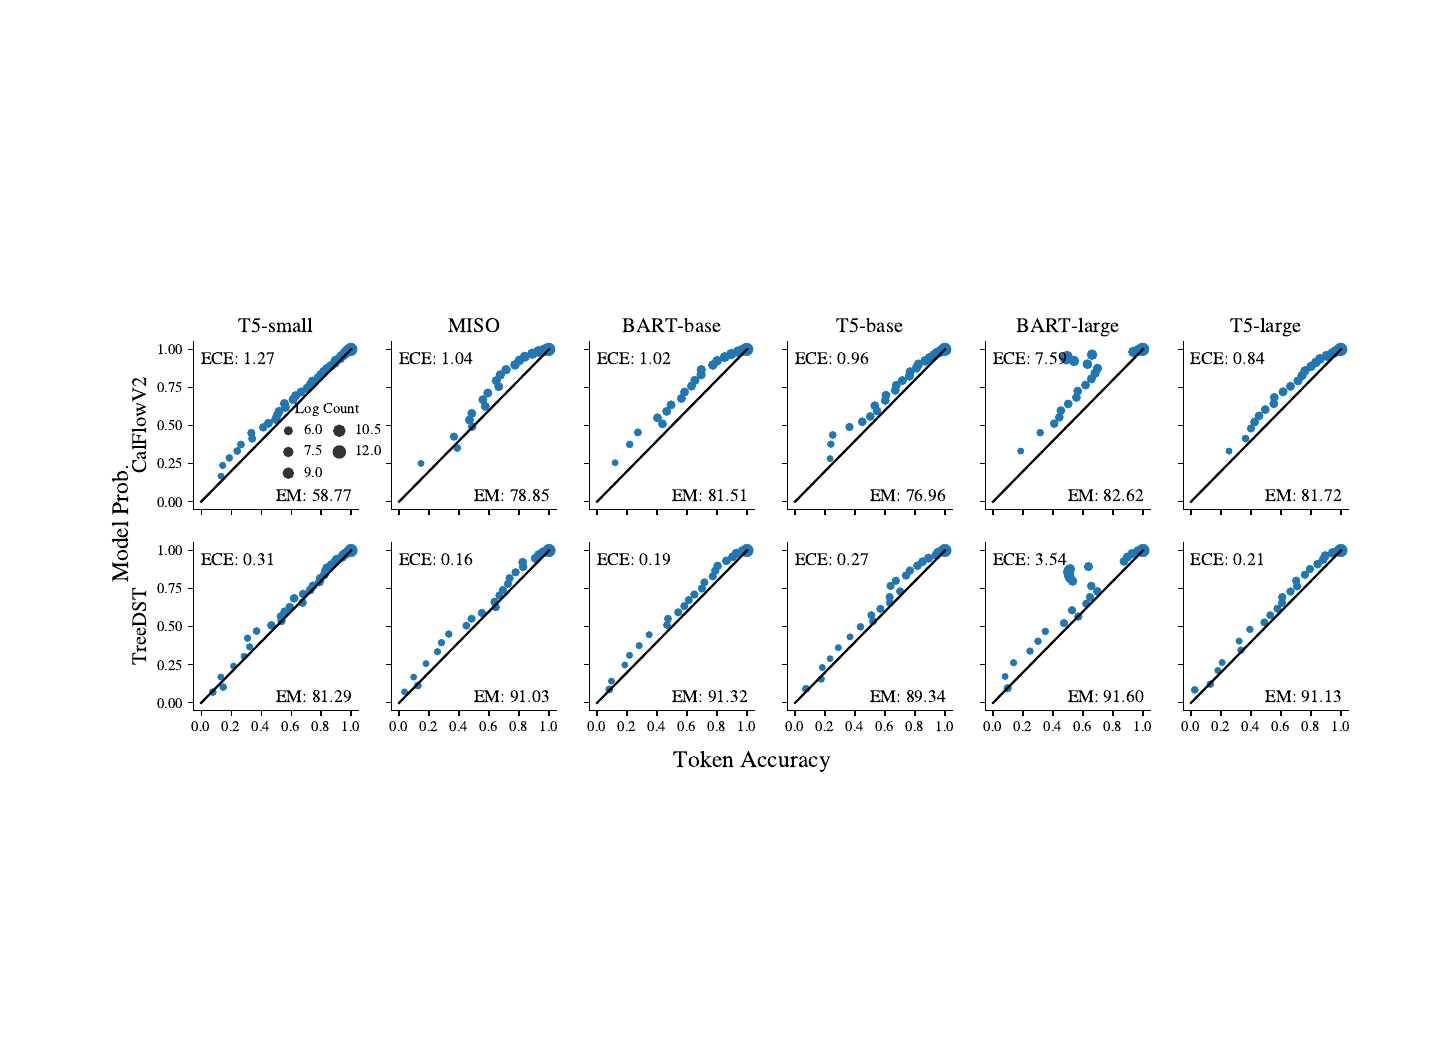
\includegraphics[width=3.363cm]{figures/img/hero_collage/tile_0.png}}};
\draw[black!35,line width=0.35pt] (0.070,-1.150) rectangle (3.433,-3.571);
\node[anchor=north west,text=ACMDarkBlue,font=\tiny\bfseries,inner sep=0] at (0.100,-3.601) {\href{https://arxiv.org/abs/2211.07443}{\adjustbox{max width=3.303cm}{Stengel-Eskin and Van Durme 2023}}};
\node[anchor=north west,text=black!60,font=\tiny,inner sep=0] at (0.100,-3.806) {\href{https://arxiv.org/abs/2211.07443}{Fig. 1, p.~6}};
\node[anchor=north west,inner sep=0] at (3.502,-1.150) {\href{https://arxiv.org/abs/2607.16799}{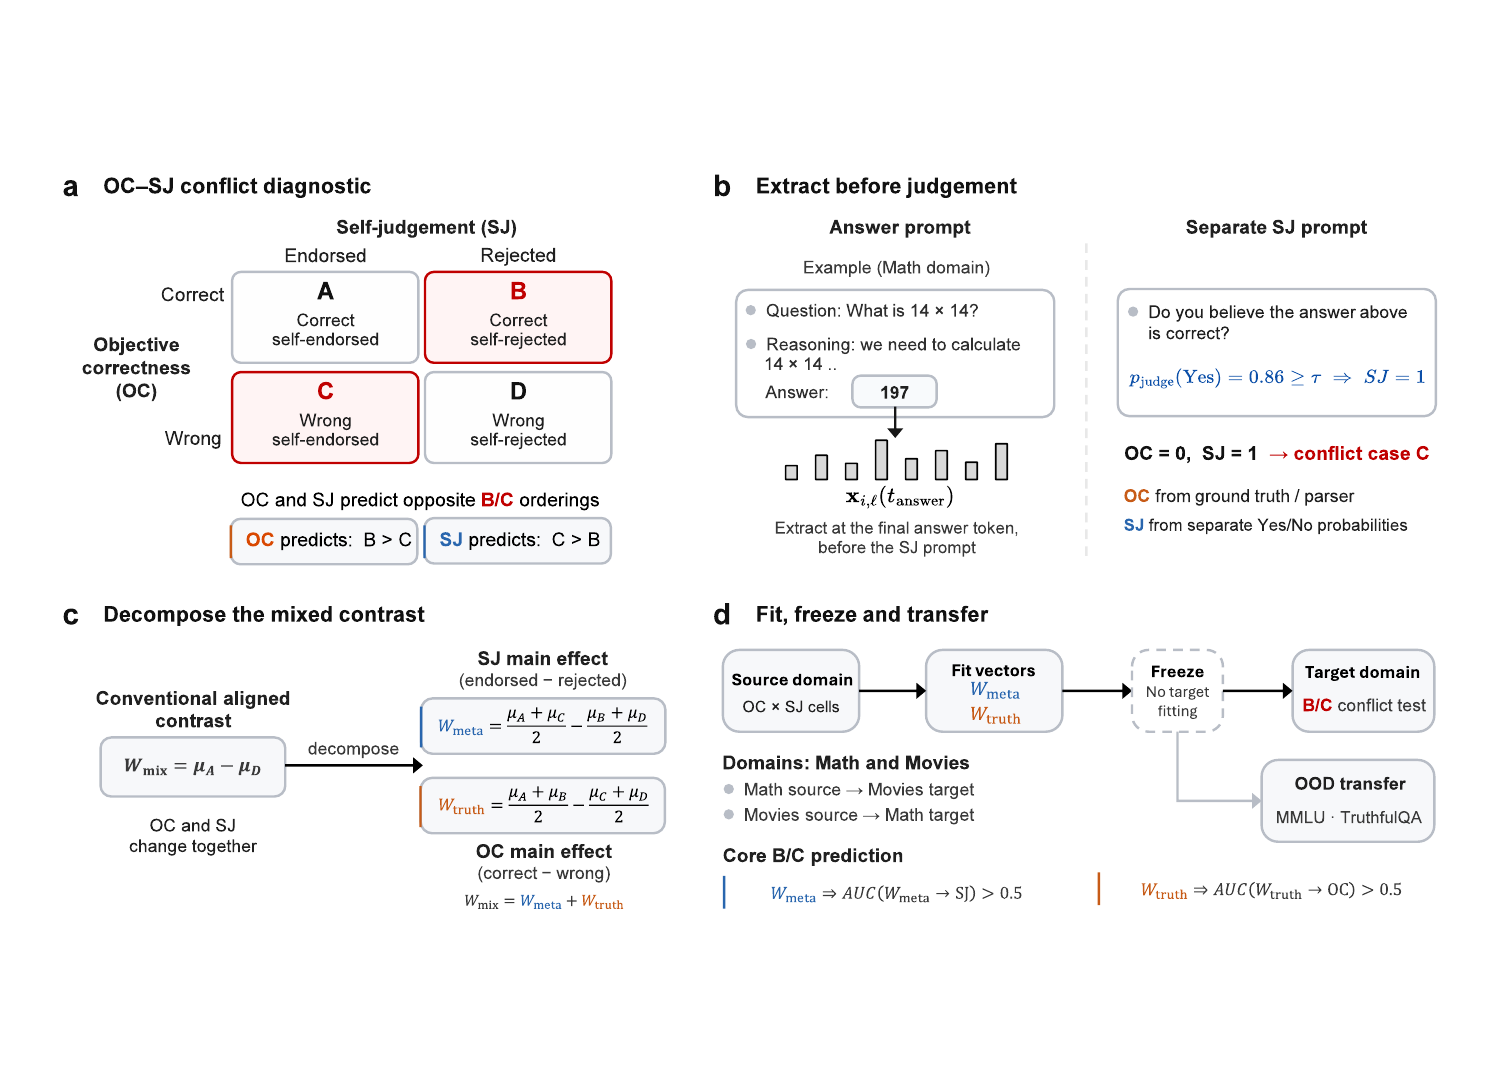
\includegraphics[width=3.363cm]{figures/img/hero_collage/tile_1.png}}};
\draw[black!35,line width=0.35pt] (3.502,-1.150) rectangle (6.865,-3.571);
\node[anchor=north west,text=ACMDarkBlue,font=\tiny\bfseries,inner sep=0] at (3.532,-3.601) {\href{https://arxiv.org/abs/2607.16799}{\adjustbox{max width=3.303cm}{Lu 2026}}};
\node[anchor=north west,text=black!60,font=\tiny,inner sep=0] at (3.532,-3.806) {\href{https://arxiv.org/abs/2607.16799}{Fig. 1, p.~2}};
\node[anchor=north west,inner sep=0] at (6.935,-1.150) {\href{https://arxiv.org/abs/2606.17234}{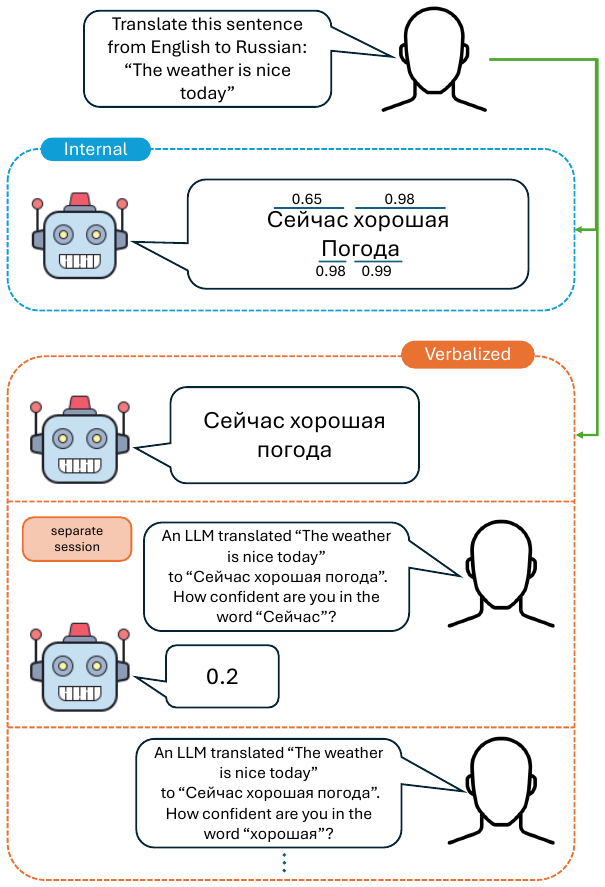
\includegraphics[width=3.363cm]{figures/img/hero_collage/tile_2.png}}};
\draw[black!35,line width=0.35pt] (6.935,-1.150) rectangle (10.298,-3.571);
\node[anchor=north west,text=ACMDarkBlue,font=\tiny\bfseries,inner sep=0] at (6.965,-3.601) {\href{https://arxiv.org/abs/2606.17234}{\adjustbox{max width=3.303cm}{Marashian et al. 2026}}};
\node[anchor=north west,text=black!60,font=\tiny,inner sep=0] at (6.965,-3.806) {\href{https://arxiv.org/abs/2606.17234}{Fig. 1, p.~1}};
\node[anchor=north west,inner sep=0] at (10.367,-1.150) {\href{https://arxiv.org/abs/2505.09427}{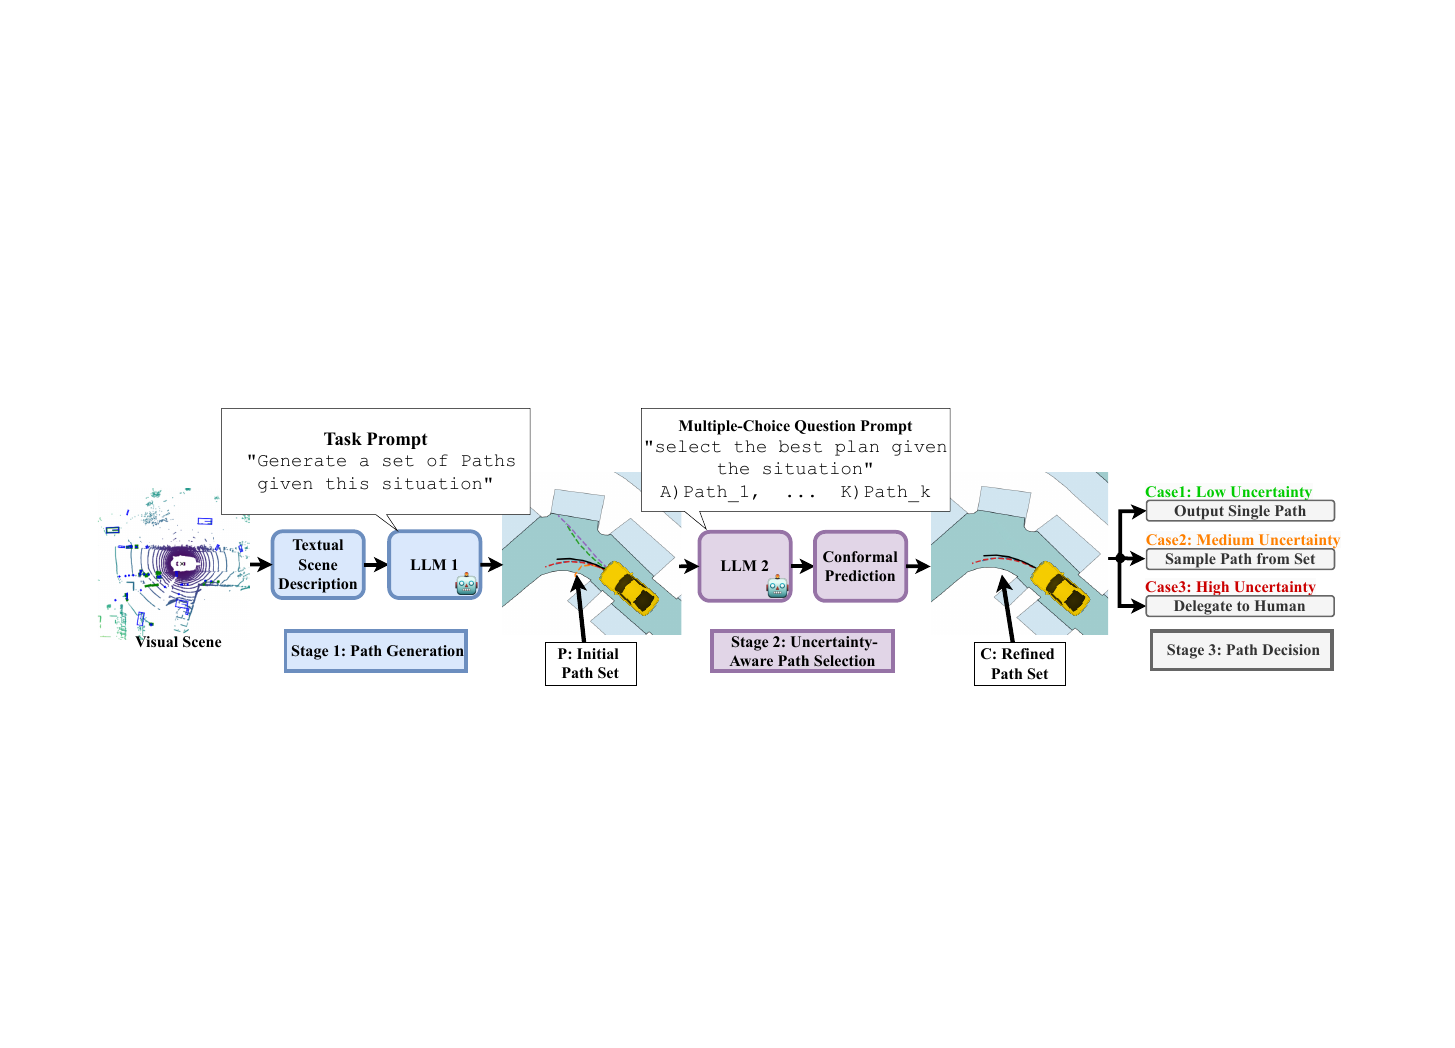
\includegraphics[width=3.363cm]{figures/img/hero_collage/tile_3.png}}};
\draw[black!35,line width=0.35pt] (10.367,-1.150) rectangle (13.730,-3.571);
\node[anchor=north west,text=ACMDarkBlue,font=\tiny\bfseries,inner sep=0] at (10.397,-3.601) {\href{https://arxiv.org/abs/2505.09427}{\adjustbox{max width=3.303cm}{Doula et al. 2025}}};
\node[anchor=north west,text=black!60,font=\tiny,inner sep=0] at (10.397,-3.806) {\href{https://arxiv.org/abs/2505.09427}{Fig. 1, p.~3}};
\fill[c7C5471] (0,-4.061) rectangle (13.800,-4.561);
\node[anchor=west,text=white,font=\footnotesize\bfseries,inner sep=0] at (0.14,-4.311) {Trained into the model: a calibration term in the training loss or reward (S4)};
\node[anchor=north west,inner sep=0] at (1.786,-4.631) {\href{https://arxiv.org/abs/2607.01612}{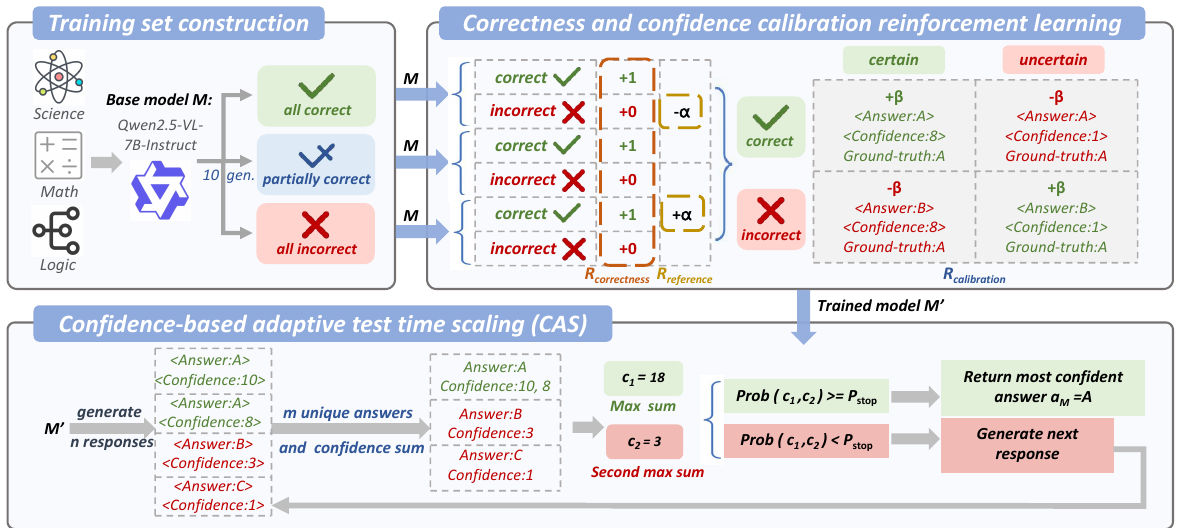
\includegraphics[width=3.363cm]{figures/img/hero_collage/tile_4.png}}};
\draw[black!35,line width=0.35pt] (1.786,-4.631) rectangle (5.149,-7.052);
\node[anchor=north west,text=ACMDarkBlue,font=\tiny\bfseries,inner sep=0] at (1.816,-7.082) {\href{https://arxiv.org/abs/2607.01612}{\adjustbox{max width=3.303cm}{Yang et al. 2026b}}};
\node[anchor=north west,text=black!60,font=\tiny,inner sep=0] at (1.816,-7.287) {\href{https://arxiv.org/abs/2607.01612}{Fig. 1, p.~3}};
\node[anchor=north west,inner sep=0] at (5.219,-4.631) {\href{https://arxiv.org/abs/2604.05306}{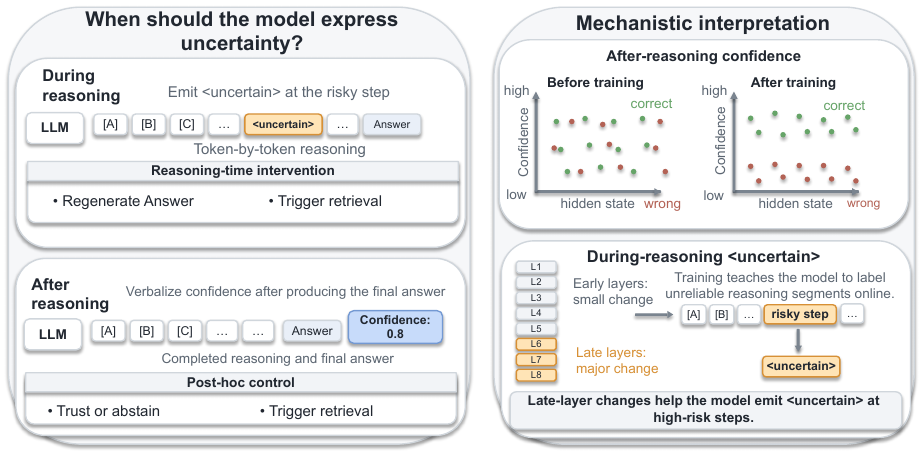
\includegraphics[width=3.363cm]{figures/img/hero_collage/tile_5.png}}};
\draw[black!35,line width=0.35pt] (5.219,-4.631) rectangle (8.581,-7.052);
\node[anchor=north west,text=ACMDarkBlue,font=\tiny\bfseries,inner sep=0] at (5.249,-7.082) {\href{https://arxiv.org/abs/2604.05306}{\adjustbox{max width=3.303cm}{Guo et al. 2026}}};
\node[anchor=north west,text=black!60,font=\tiny,inner sep=0] at (5.249,-7.287) {\href{https://arxiv.org/abs/2604.05306}{Fig. 1, p.~2}};
\node[anchor=north west,inner sep=0] at (8.651,-4.631) {\href{https://arxiv.org/abs/2604.22779}{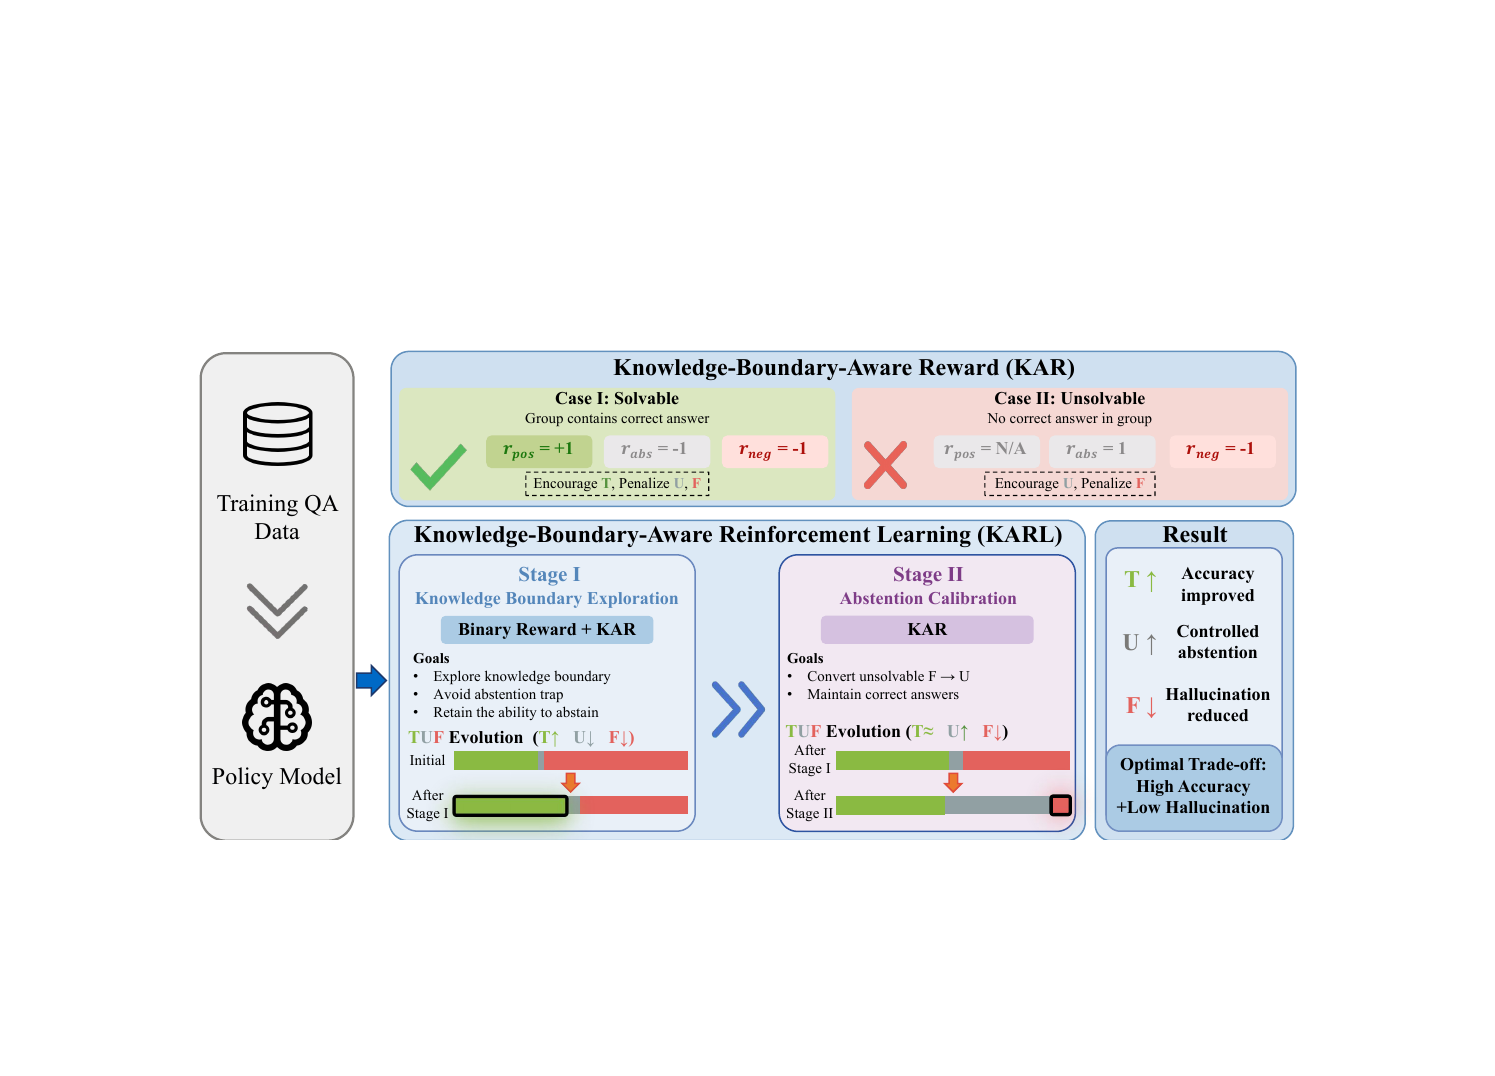
\includegraphics[width=3.363cm]{figures/img/hero_collage/tile_6.png}}};
\draw[black!35,line width=0.35pt] (8.651,-4.631) rectangle (12.014,-7.052);
\node[anchor=north west,text=ACMDarkBlue,font=\tiny\bfseries,inner sep=0] at (8.681,-7.082) {\href{https://arxiv.org/abs/2604.22779}{\adjustbox{max width=3.303cm}{Gao et al. 2026}}};
\node[anchor=north west,text=black!60,font=\tiny,inner sep=0] at (8.681,-7.287) {\href{https://arxiv.org/abs/2604.22779}{Fig. 4, p.~4}};
\end{tikzpicture}}
\caption{\textbf{Confidence estimated after the fact, and confidence trained into the model.} Panels are drawn from Figures~\ref{fig:method_gallery} and~\ref{fig:results_gallery} under the same licence rule: one per stage for S0, S1, S2, S3, and one per training family for S4 (T1, T3, T4; T2, T5 not shown). Each label links to the paper; Table~\ref{tab:panel_provenance} gives the figure, page and licence.}
\Description{A labelled grid of images, each a hyperlink annotated with its system name and source figure number.}
\label{fig:hero_collage}
\end{figure*}



This survey maps calibration-aware decision-making with language models, with the training stage as
its core. We place each of \nWorks works by the stage at which calibration enters the decision
pipeline (Table~\ref{tab:definitions}), organise the \nCore training-stage works by what the training
signal scores, and classify every work by the \emph{output contract} its confidence is attached to:
a typed decision with a probability per declared option, a prediction set, constrained output, a single
confidence score, or free text. The two classifications meet in one finding: of the \nContractTyped works
that attach the confidence to a typed decision, most calibrate a classifier or a multiple-choice
read-off after the fact, and only \nCoreTyped of the \nCore training works train one
(Section~\ref{sec:contract}).

\paragraph{Contributions.} This survey offers the following.
\begin{itemize}
  \item A \textbf{stage taxonomy} of \nWorks works (Figure~\ref{fig:taxonomy_main} shows \nTaxShown of them), with operational
        placement rules (Table~\ref{tab:definitions}) and a per-work record of stage, output contract,
        access, guarantee, metric and action (Tables~\ref{tab:compare_s4} and~\ref{tab:landscape}).
  \item A \textbf{typology of calibration training}: the \nCore training-stage works in five families
        by what the training signal scores (Section~\ref{sec:core}, Table~\ref{tab:compare_s4}), and
        what each stage yields, costs and guarantees (Table~\ref{tab:stage_limits}).
  \item A \textbf{coverage comparison} with the \nSurveysCompared closest prior surveys
        (Table~\ref{tab:survey_compare}, Figure~\ref{fig:survey_timeline}), and a profile of the corpus
        (Figures~\ref{fig:corpus_overview} to~\ref{fig:results_gallery}), every gallery panel
        traced to its source figure and licence (Table~\ref{tab:panel_provenance}).
  \item An analysis of the \textbf{output contract and the decision loop} (Section~\ref{sec:contract},
        Figure~\ref{fig:decision_loop}, Table~\ref{tab:compare_contract}).
  \item A \textbf{measurable agenda}: seven quantities with named public testbeds
        (Table~\ref{tab:future_metrics}), with the calibration of the decision itself measured for the
        \nDISystems systems of a public leaderboard (Figure~\ref{fig:future_protocol}).
\end{itemize}

% AUTO-GENERATED by build/gen_taxonomy.py from literature/corpus.tsv -- do not hand-edit.
\begin{figure*}[p]
\centering
\resizebox{!}{0.84\textheight}{%
\begin{forest}
  for tree={align=center},
  where n children=0{font=\footnotesize, align=left}{font=\normalsize},
  where level=1{font=\large}{},
  where level=0{font=\Large}{},
[\textbf{Calibration-aware}\\\textbf{decision-making}\\\textbf{with language}\\\textbf{models}, fill=black!8, text width=12em
  [\textbf{S0 read-off}, fill=stS0!40, text width=9em
    [\textbf{Calibration after}\\\textbf{alignment}, fill=stS0!22, text width=12.5em
      [{\textbf{OpenAI}: GPT-4 Technical Report~\citep{openai2023gpt4}\\\textbf{Sanz-Guerrero}: Large Language Models Are\ldots~\citep{sanzguerrero2026large}}, fill=stS0!7, text width=40em, align=left]
    ]
    [\textbf{Empirical studies of}\\\textbf{read-off calibration}, fill=stS0!22, text width=12.5em
      [{\textbf{Desai}: Calibration of Pre-trained Transformers~\citep{desai2020calibration}\\\textbf{Calibration Across Layers}: Understanding Calibration\ldots~\citep{joshi2025calibration}}, fill=stS0!7, text width=40em, align=left]
    ]
    [\textbf{Likelihood and logit}\\\textbf{read-off}, fill=stS0!22, text width=12.5em
      [{\textbf{Ott}: Analyzing Uncertainty in Neural Machine Translation~\citep{ott2018analyzing}\\\textbf{My Answer is C}: First-Token Probabilities Do Not Match\ldots~\citep{wang2024my}}, fill=stS0!7, text width=40em, align=left]
    ]
    [\textbf{Self-evaluation and}\\\textbf{read-off calibration}, fill=stS0!22, text width=12.5em
      [{\textbf{Kadavath}: Language Models (Mostly) Know What They Know~\citep{kadavath2022language}}, fill=stS0!7, text width=40em, align=left]
    ]
  ]
  [\textbf{S1 post-hoc}\\\textbf{map}, fill=stS1!40, text width=9em
    [\textbf{Fixed maps over the}\\\textbf{read-off}, fill=stS1!22, text width=12.5em
      [{\textbf{Zhang}: Enhancing Uncertainty-Based Hallucination Detection\ldots~\citep{zhang2023enhancing}\\\textbf{The Silent Vote}: Improving Zero-Shot LLM Reliability by\ldots~\citep{badhe2026silent}}, fill=stS1!7, text width=40em, align=left]
    ]
    [\textbf{Label-bias and}\\\textbf{option-prior}\\\textbf{debiasing}, fill=stS1!22, text width=12.5em
      [{\textbf{Zheng}: Large Language Models Are Not Robust Multiple Choice\ldots~\citep{zheng2023large}\\\textbf{Beyond Performance}: Quantifying and Mitigating Label Bias\ldots~\citep{reif2024beyond}}, fill=stS1!7, text width=40em, align=left]
    ]
    [\textbf{Learned calibrators}, fill=stS1!22, text width=12.5em
      [{\textbf{Ye}: Can Explanations Be Useful for Calibrating Black Box Models?~\citep{ye2021can}\\\textbf{Luo}: Unlocking the Pre-Trained Model as a Dual-Alignment\ldots~\citep{luo2026unlocking}}, fill=stS1!7, text width=40em, align=left]
    ]
    [\textbf{Multicalibration and}\\\textbf{task-specific}\\\textbf{recalibration}, fill=stS1!22, text width=12.5em
      [{\textbf{Detommaso}: Multicalibration for Confidence Scoring in\ldots~\citep{detommaso2024multicalibration}\\\textbf{Liu}: On Calibration of LLM-based Guard Models for Reliable\ldots~\citep{liu2024calibration}}, fill=stS1!7, text width=40em, align=left]
    ]
    [\textbf{Probes and learned}\\\textbf{confidence heads}, fill=stS1!22, text width=12.5em
      [{\textbf{Kumar}: Calibration of Encoder Decoder Models for Neural\ldots~\citep{kumar2019calibration}\\\textbf{Lu}: Diagnosing Correctness Probes under Self-Judgement\ldots~\citep{lu2026diagnosing}}, fill=stS1!7, text width=40em, align=left]
    ]
    [\textbf{Prompt and context}\\\textbf{calibration}, fill=stS1!22, text width=12.5em
      [{\textbf{Surface Form Competition}: Why the Highest Probability\ldots~\citep{holtzman2021surface}\\\textbf{Gundem}: Boosting In-Context Learning in LLMs Through the\ldots~\citep{gundem2025boosting}}, fill=stS1!7, text width=40em, align=left]
    ]
    [\textbf{Scaling and binning}, fill=stS1!22, text width=12.5em
      [{\textbf{Guo}: On Calibration of Modern Neural Networks~\citep{guo2017calibration}\\\textbf{Luo}: Your Pre-trained LLM is Secretly an Unsupervised\ldots~\citep{luo2025your}}, fill=stS1!7, text width=40em, align=left]
    ]
  ]
  [\textbf{S2 prompt}\\\textbf{elicitation}, fill=stS2!40, text width=9em
    [\textbf{Abstention prompting}, fill=stS2!22, text width=12.5em
      [{\textbf{I-CALM}: Incentivizing Confidence-Aware Abstention for LLM\ldots~\citep{zong2026icalm}}, fill=stS2!7, text width=40em, align=left]
    ]
    [\textbf{Introspection,}\\\textbf{deliberation and}\\\textbf{task-specific}\\\textbf{elicitation}, fill=stS2!22, text width=12.5em
      [{\textbf{Sun}: Confidence Estimation for LLM-Based Dialogue State Tracking~\citep{sun2024confidence}\\\textbf{Reasoning about Uncertainty}: Do Reasoning Models Know\ldots~\citep{mei2025reasoning}}, fill=stS2!7, text width=40em, align=left]
    ]
    [\textbf{Linguistic hedges and}\\\textbf{epistemic markers}, fill=stS2!22, text width=12.5em
      [{\textbf{Sileo}: Probing neural language models for understanding of\ldots~\citep{sileo2022probing}\\\textbf{Liu}: Can LLMs Use Linguistic Uncertainty Markers to Reliably\ldots~\citep{liu2026can}}, fill=stS2!7, text width=40em, align=left]
    ]
    [\textbf{Self-evaluation}\\\textbf{prompts}, fill=stS2!22, text width=12.5em
      [{\textbf{Tian}: Overconfidence in LLM-as-a-Judge: Diagnosis and\ldots~\citep{tian2025overconfidence}}, fill=stS2!7, text width=40em, align=left]
    ]
    [\textbf{Stated confidence}\\\textbf{that triggers an}\\\textbf{action}, fill=stS2!22, text width=12.5em
      [{\textbf{Ni}: When Do LLMs Need Retrieval Augmentation? Mitigating LLMs'\ldots~\citep{ni2024when}\\\textbf{Ferrer}: When Can We Trust LLM Graders? Calibrating\ldots~\citep{ferrer2026when}}, fill=stS2!7, text width=40em, align=left]
    ]
    [\textbf{Verbalised numeric}\\\textbf{confidence}, fill=stS2!22, text width=12.5em
      [{\textbf{Tanneru}: Quantifying Uncertainty in Natural Language\ldots~\citep{tanneru2023quantifying}\\\textbf{Yang}: The Mirage of Calibrated Confidence\ldots~\citep{yang2026the}}, fill=stS2!7, text width=40em, align=left]
    ]
  ]
  [\textbf{S3 extra}\\\textbf{inference}, fill=stS3!40, text width=9em
    [\textbf{Benchmarks and}\\\textbf{empirical studies}, fill=stS3!22, text width=12.5em
      [{\textbf{LM-Polygraph}: Uncertainty Estimation for Language Models~\citep{fadeeva2023lmpolygraph}\\\textbf{Vashurin}: Benchmarking Uncertainty Quantification\ldots~\citep{vashurin2024benchmarking}}, fill=stS3!7, text width=40em, align=left]
    ]
    [\textbf{Conformal abstention,}\\\textbf{selection and}\\\textbf{cascades}, fill=stS3!22, text width=12.5em
      [{\textbf{Fisch}: Efficient Conformal Prediction via Cascaded\ldots~\citep{fisch2020efficient}\\\textbf{Tayebati}: Learning Conformal Abstention Policies for\ldots~\citep{tayebati2025learning}}, fill=stS3!7, text width=40em, align=left]
    ]
    [\textbf{Conformal factuality}\\\textbf{and claim filtering}, fill=stS3!22, text width=12.5em
      [{\textbf{Cherian}: Large language model validity via enhanced\ldots~\citep{cherian2024large}\\\textbf{Rubin-Toles}: Conformal Language Model Reasoning with\ldots~\citep{rubintoles2025conformal}}, fill=stS3!7, text width=40em, align=left]
    ]
    [\textbf{Conformal prediction}\\\textbf{sets}, fill=stS3!22, text width=12.5em
      [{\textbf{Dey}: Conformal prediction for text infilling and\ldots~\citep{dey2021conformal}\\\textbf{CommCP}: Efficient Multi-Agent Coordination via LLM-Based\ldots~\citep{zhang2026commcp}}, fill=stS3!7, text width=40em, align=left]
    ]
    [\textbf{Ensembles and}\\\textbf{cross-model}\\\textbf{disagreement}, fill=stS3!22, text width=12.5em
      [{\textbf{Dong}: Confidence Modeling for Neural Semantic Parsing~\citep{dong2018confidence}\\\textbf{Hamidieh}: Complementing Self-Consistency with\ldots~\citep{hamidieh2026complementing}}, fill=stS3!7, text width=40em, align=left]
    ]
    [\textbf{Internal-state}\\\textbf{signals}, fill=stS3!22, text width=12.5em
      [{\textbf{Fomicheva}: Unsupervised Quality Estimation for Neural\ldots~\citep{fomicheva2020unsupervised}\\\textbf{Semantic Volume}: Quantifying and Detecting both External and\ldots~\citep{li2025semantic}}, fill=stS3!7, text width=40em, align=left]
    ]
    [\textbf{Long-form and}\\\textbf{claim-level}, fill=stS3!22, text width=12.5em
      [{\textbf{Da}: LLM Uncertainty Quantification through Directional\ldots~\citep{da2024llm}\\\textbf{IUQ}: Interrogative Uncertainty Quantification for Long-Form\ldots~\citep{fan2026iuq}}, fill=stS3!7, text width=40em, align=left]
    ]
    [\textbf{Risk control and}\\\textbf{early exit}, fill=stS3!22, text width=12.5em
      [{\textbf{Learn then Test}: Calibrating Predictive Algorithms\ldots~\citep{angelopoulos2021learn}\\\textbf{Conformal Thinking}: Risk Control for Reasoning on a\ldots~\citep{wang2026conformal}}, fill=stS3!7, text width=40em, align=left]
    ]
    [\textbf{Sampling consistency}, fill=stS3!22, text width=12.5em
      [{\textbf{Wang}: Self-Consistency Improves Chain of Thought Reasoning\ldots~\citep{wang2022selfconsistency}\\\textbf{Too Consistent to Detect}: A Study of Self-Consistent\ldots~\citep{tan2025too}}, fill=stS3!7, text width=40em, align=left]
    ]
    [\textbf{Semantic entropy and}\\\textbf{meaning clustering}, fill=stS3!22, text width=12.5em
      [{\textbf{Semantic Uncertainty}: Linguistic Invariances for\ldots~\citep{kuhn2023semantic}\\\textbf{Sun}: Efficient Hallucination Detection: Adaptive Bayesian\ldots~\citep{sun2026efficient}}, fill=stS3!7, text width=40em, align=left]
    ]
    [\textbf{Token-level}\\\textbf{aggregation}, fill=stS3!22, text width=12.5em
      [{\textbf{Malinin}: Uncertainty Estimation in Autoregressive\ldots~\citep{malinin2020uncertainty}\\\textbf{Word-Sequence Entropy}: Towards Uncertainty Estimation in\ldots~\citep{wang2024wordsequence}}, fill=stS3!7, text width=40em, align=left]
    ]
  ]
  [\textbf{S4 training}, fill=stS4!40, text width=9em
    [\textbf{T1 supervised}\\\textbf{calibration}\\\textbf{objectives}, fill=stS4!30, text width=10.5em
      [{\textbf{Jiang}: How Can We Know When Language Models Know? On the\ldots~\citep{jiang2020how}\\\textbf{Chaudhry}: Finetuning Language Models to Emit Linguistic\ldots~\citep{chaudhry2024finetuning}\\\textbf{Kapoor}: Large Language Models Must Be Taught to Know What\ldots~\citep{kapoor2024large}\\\textbf{Niu}: Functional-level Uncertainty Quantification for\ldots~\citep{niu2024functionallevel}\\\textbf{Uncertainty Distillation}: Teaching Language Models to\ldots~\citep{hager2025uncertainty}\\\textbf{ConfTuner}: Training Large Language Models to Express Their\ldots~\citep{li2025conftuner}\\\textbf{Direct Confidence Alignment}: Aligning Verbalized\ldots~\citep{zhang2025direct}\\\textbf{Know When You're Wrong}: Aligning Confidence with\ldots~\citep{xiaohu2026know}}, fill=stS4!8, text width=40em, align=left]
    ]
    [\textbf{T2 reward-model}\\\textbf{calibration}, fill=stS4!30, text width=10.5em
      [{\textbf{Leng}: Taming Overconfidence in LLMs: Reward Calibration in RLHF~\citep{leng2024taming}\\\textbf{Lou}: Uncertainty-aware Reward Model: Teaching Reward Models\ldots~\citep{lou2024uncertaintyaware}\\\textbf{Know What You Don't Know}: Uncertainty Calibration of\ldots~\citep{park2025know}\\\textbf{Ma}: Distributional Process Reward Models: Calibrated\ldots~\citep{ma2026distributional}\\\textbf{Pan}: Uncertainty-Aware Reward Modeling for Stable RLHF~\citep{pan2026uncertaintyaware}}, fill=stS4!8, text width=40em, align=left]
    ]
    [\textbf{T3 calibration}\\\textbf{rewards on the}\\\textbf{stated confidence}, fill=stS4!30, text width=10.5em
      [{\textbf{Band}: Linguistic Calibration of Long-Form Generations~\citep{band2024linguistic}\\\textbf{Rewarding Doubt}: A Reinforcement Learning Approach\ldots~\citep{baniharouni2025rewarding}\\\textbf{Niekerk}: Post-Training Large Language Models via\ldots~\citep{vanniekerk2025posttraining}\\\textbf{Zou}: Thinking, Faithful and Stable: Mitigating Hallucinations\ldots~\citep{zou2025thinking}\\\textbf{ORCE}: Order-Aware Alignment of Verbalized Confidence in Large\ldots~\citep{li2026orce}\\\textbf{Singh}: Verifiable Rewards for Calibrated Probabilistic\ldots~\citep{singh2026verifiable}\\\textbf{DualStake}: Dual-Path Confidence Calibration in Deep Research\ldots~\citep{xu2026dualstake}\\\textbf{Closing the Reflection Gap}: A Free Calibration Bonus for\ldots~\citep{zhu2026closing}}, fill=stS4!8, text width=40em, align=left]
    ]
    [\textbf{T4 abstention and}\\\textbf{refusal training}, fill=stS4!30, text width=10.5em
      [{\textbf{Yang}: Alignment for Honesty~\citep{yang2023alignment}\\\textbf{Chen}: Teaching Large Language Models to Express Knowledge\ldots~\citep{chen2024teaching}\\\textbf{Know the Unknown}: An Uncertainty-Sensitive Method for LLM\ldots~\citep{li2024know}\\\textbf{Xu}: Rejection Improves Reliability: Training LLMs to Refuse\ldots~\citep{xu2024rejection}\\\textbf{Honesty over Accuracy}: Trustworthy Language Models\ldots~\citep{mohamadi2025honesty}\\\textbf{TruthRL}: Incentivizing Truthful LLMs via Reinforcement Learning~\citep{wei2025truthrl}\\\textbf{TIAR}: Trajectory-Informed Advantage Reweighting for LLM\ldots~\citep{pan2026tiar}\\\textbf{Abstain-R1}: Calibrated Abstention and Post-Refusal\ldots~\citep{zhai2026abstainr1}}, fill=stS4!8, text width=40em, align=left]
    ]
    [\textbf{T5 process- and}\\\textbf{meaning-level}\\\textbf{confidence rewards}, fill=stS4!30, text width=10.5em
      [{\textbf{An}: Teaching LLMs to Abstain via Fine-Grained Semantic\ldots~\citep{an2025teaching}\\\textbf{MMBoundary}: Advancing MLLM Knowledge Boundary Awareness\ldots~\citep{he2025mmboundary}\\\textbf{Wang}: Process Supervision of Confidence Margin for\ldots~\citep{wang2026process}\\\textbf{Yu}: Calibrating LLMs with Semantic-level Reward~\citep{yu2026calibrating}}, fill=stS4!8, text width=40em, align=left]
    ]
  ]
  [\textbf{Theory and}\\\textbf{analysis}, fill=stTH!40, text width=9em
    [{\textbf{Błasiok}: When Does Optimizing a Proper Loss Yield\ldots~\citep{blasiok2023when}\\\textbf{Kalai}: Calibrated Language Models Must Hallucinate~\citep{kalai2023calibrated}\\\textbf{Uncalibrated Reasoning}: GRPO Induces Overconfidence\ldots~\citep{bereket2025uncalibrated}\\\textbf{Kalai}: Why Language Models Hallucinate~\citep{kalai2025why}\\\textbf{Nakkiran}: Trained on Tokens, Calibrated on Concepts\ldots~\citep{nakkiran2025trained}}, fill=stTH!15, text width=40em, align=left]
  ]
  [\textbf{X consumers}\\\textbf{and contract}, fill=stX!40, text width=9em
    [\textbf{Abstention}, fill=stX!22, text width=12.5em
      [{\textbf{Kamath}: Selective Question Answering under Domain Shift~\citep{kamath2020selective}\\\textbf{Srinivasan}: Selective "Selective Prediction"\ldots~\citep{srinivasan2024selective}}, fill=stX!7, text width=40em, align=left]
    ]
    [\textbf{Adaptive compute}, fill=stX!22, text width=12.5em
      [{\textbf{Let's Sample Step by Step}: Adaptive-Consistency for\ldots~\citep{aggarwal2023lets}\\\textbf{Yang}: Dynamic Early Exit in Reasoning Models~\citep{yang2025dynamic}}, fill=stX!7, text width=40em, align=left]
    ]
    [\textbf{Confidence-weighted}\\\textbf{selection}, fill=stX!22, text width=12.5em
      [{\textbf{Taubenfeld}: Confidence Improves Self-Consistency in LLMs~\citep{taubenfeld2025confidence}}, fill=stX!7, text width=40em, align=left]
    ]
    [\textbf{Constrained decoding}, fill=stX!22, text width=12.5em
      [{\textbf{PICARD}: Parsing Incrementally for Constrained\ldots~\citep{scholak2021picard}\\\textbf{Reddy}: The Hidden Cost of Structured Generation in LLMs\ldots~\citep{reddy2026hidden}}, fill=stX!7, text width=40em, align=left]
    ]
    [\textbf{Deferral}, fill=stX!22, text width=12.5em
      [{\textbf{Jitkrittum}: When Does Confidence-Based Cascade\ldots~\citep{jitkrittum2023when}\\\textbf{L2D-Clinical}: Learning to Defer for Adaptive Model\ldots~\citep{kondadadi2026l2dclinical}}, fill=stX!7, text width=40em, align=left]
    ]
    [\textbf{Human reliance on}\\\textbf{model output and}\\\textbf{stated confidence}, fill=stX!22, text width=12.5em
      [{\textbf{Si}: Large Language Models Help Humans Verify Truthfulness --\ldots~\citep{si2023large}\\\textbf{Not All Uncertainty Is Equal}: How Uncertainty\ldots~\citep{villavicencio2026not}}, fill=stX!7, text width=40em, align=left]
    ]
    [\textbf{Judge calibration}, fill=stX!22, text width=12.5em
      [{\textbf{Liu}: Calibrating LLM-Based Evaluator~\citep{liu2023calibrating}\\\textbf{JEV-as-a-Judge}: Accept When Confident, Escalate When Unsure~\citep{li2026jev}}, fill=stX!7, text width=40em, align=left]
    ]
    [\textbf{Routing/cascade}, fill=stX!22, text width=12.5em
      [{\textbf{Model Cascading}: Towards Jointly Improving Efficiency\ldots~\citep{varshney2022model}\\\textbf{Bouchard}: Is Escalation Worth It? A Decision-Theoretic\ldots~\citep{bouchard2026is}}, fill=stX!7, text width=40em, align=left]
    ]
    [\textbf{Structured-output}\\\textbf{benchmark}, fill=stX!22, text width=12.5em
      [{\textbf{Struc-Bench}: Are Large Language Models Really Good at\ldots~\citep{tang2023strucbench}\\\textbf{Singh}: The Structured Output Benchmark: A Multi-Source\ldots~\citep{singh2026structured}}, fill=stX!7, text width=40em, align=left]
    ]
    [\textbf{Studies and}\\\textbf{benchmarks of}\\\textbf{abstention}, fill=stX!22, text width=12.5em
      [{\textbf{Tomani}: Uncertainty-Based Abstention in LLMs Improves\ldots~\citep{tomani2024uncertaintybased}\\\textbf{Wang}: Are LLM Decisions Faithful to Verbal Confidence?~\citep{wang2026are}}, fill=stX!7, text width=40em, align=left]
    ]
    [\textbf{Typed classification}, fill=stX!22, text width=12.5em
      [{\textbf{Look at the Text}: Instruction-Tuned Language Models are\ldots~\citep{wang2024look}}, fill=stX!7, text width=40em, align=left]
    ]
  ]
]
\end{forest}}
\caption{\textbf{A taxonomy of calibration-aware decision-making with language models} (111 of the 408
works in Tables~\ref{tab:compare_s4} and~\ref{tab:landscape}). Branches are the stage at which calibration enters (Table~\ref{tab:definitions}); X holds
the works that consume a confidence or fix the output contract. The core, S4 (80 works), is grouped by what the
training signal scores and lists up to 8 works per family, evenly spaced over the family's works in year order
(33 shown; all are in Table~\ref{tab:compare_s4}). The 5 theory and analysis works are listed in
full and are not counted in the core. Every other family lists its earliest and its latest work. Each line gives a trimmed form
of the paper's own title; a citation may show a later venue year than the first-version year counted in
Figures~\ref{fig:corpus_dist} and~\ref{fig:stage_trend}.}
\Description{A tree diagram rooted at calibration-aware decision-making with language models, with branches for read-off,
post-hoc maps, prompt elicitation, extra inference, training (split into five families by what the training signal scores),
theory and analysis, and consumers and output contract. Each family cell lists papers with short titles.}
\label{fig:taxonomy_main}
\end{figure*}


\subsection{Related surveys and the empty cell}
\label{sec:related}

Table~\ref{tab:survey_compare} (Appendix~\ref{app:surveys}) compares the \nSurveysCompared closest prior surveys on seven topics:
confidence estimation and calibration, calibration-aware training of any kind, reinforcement learning
whose reward is a calibration or proper-scoring-rule objective, decisions over a predefined option set,
typed per-option decision outputs, acting on confidence, and hallucination.
Figure~\ref{fig:survey_timeline} places them on a timeline; \nSurveysRecent of the \nSurveysCompared
appeared from 2024 onward.


Calibration and uncertainty are well surveyed, and the stage view itself, which organises methods by
where the confidence comes from, is established~\citep{li2025survey,shorinwa2025survey}; we use it as
the frame for the background stages and credit it there. The training stage is the thinner cell. Only
\nRLRFull surveys give full coverage to reinforcement learning with a calibration reward, and each is
scoped to one slice: \citet{li2025survey} to the 2024 methods, \citet{xu2026llm} to forecasting, where
it organises calibration training by reward and maps forecast forms to proper scores, and
\citet{lin2026uncertainty} to agents, where it splits rewards by their target. \citet{ulmer2025anthropomimetic}
labels papers by the register of the confidence, numeric or verbal, and by how it is elicited: by prompting,
supervised fine-tuning or reinforcement learning. What none of the \nSurveys
surveys we identified does is organise calibration training \emph{across domains} by what the training signal scores,
or cross that typology with the output contract the confidence is trained into; no survey cites more
than one of the \nCoreFourteen general-domain calibration-training works from 2025 and 2026 that anchor
our core (marked in Table~\ref{tab:compare_s4}). Two recent non-survey works come closest: an application
paper that compares reinforcement-learning training paradigms by their signal source for one
domain~\citep{barbosa2026calibrated}, and a position paper that groups ternary-reward abstention works, three of them in
our core, in one row~\citep{ravikumar2026missing}; neither proposes a typology of training signals or an output contract. Typed per-option decision output is the emptiest column of Table~\ref{tab:survey_compare}:
no survey covers it in full.

% AUTO-GENERATED by build/gen_phaseA.py -- do not hand-edit.
\begin{figure*}[t]
\centering
\begin{tikzpicture}[font=\scriptsize]
\fill[black!4] (0,1.63) rectangle (9.90,-1.63);
\fill[black!4] (0,-1.76) rectangle (9.90,-3.16);
\fill[black!4] (0,-3.29) rectangle (9.90,-4.69);
\fill[black!4] (0,-4.82) rectangle (9.90,-6.22);
\fill[black!4] (0,-6.35) rectangle (9.90,-7.67);
\fill[black!4] (0,-7.80) rectangle (9.90,-9.12);
\draw[black!12,dashed] (0.00,1.63) -- (0.00,-9.37);
\draw[black!12,dashed] (1.65,1.63) -- (1.65,-9.37);
\draw[black!12,dashed] (3.30,1.63) -- (3.30,-9.37);
\draw[black!12,dashed] (4.95,1.63) -- (4.95,-9.37);
\draw[black!12,dashed] (6.60,1.63) -- (6.60,-9.37);
\draw[black!12,dashed] (8.25,1.63) -- (8.25,-9.37);
\node[anchor=east,align=right,text width=2.9cm,font=\scriptsize\bfseries] at (-0.15,0.00) {Calibration and uncertainty quantification};
\draw[black!35] (6.27,0.00) -- (6.27,0.36);
\draw[black!35] (6.30,0.00) -- (6.30,-0.36);
\draw[black!35] (6.49,0.00) -- (6.49,0.67);
\draw[black!35] (6.54,0.00) -- (6.54,-0.67);
\draw[black!35] (7.43,0.00) -- (7.43,0.98);
\draw[black!35] (6.96,0.00) -- (6.96,-0.98);
\draw[black!35] (7.12,0.00) -- (7.12,1.29);
\draw[black!35] (7.47,0.00) -- (7.47,-1.29);
\draw[black!35] (9.07,0.00) -- (9.07,0.36);
\draw[black!35] (8.35,0.00) -- (8.35,-0.36);
\draw[black!35] (8.40,0.00) -- (8.40,0.67);
\draw[black!35] (8.76,0.00) -- (8.76,-0.67);
\draw[black!35] (8.78,0.00) -- (8.78,-0.98);
\draw[black!35] (9.13,0.00) -- (9.13,0.98);
\draw[black!35] (9.32,0.00) -- (9.32,1.29);
\draw[black!35] (9.38,0.00) -- (9.38,-1.29);
\fill[black!75] (4.27,0.00) circle (1.6pt);
\node[anchor=south,inner sep=1.5pt,fill=black!4] at (4.27,0.05) {\href{https://arxiv.org/abs/2308.01222}{Wang 2023}};
\fill[black!75] (4.73,0.00) circle (1.6pt);
\node[anchor=north,inner sep=1.5pt,fill=black!4] at (4.73,-0.05) {\href{https://arxiv.org/abs/2311.08298}{Geng 2023}};
\fill[black!75] (6.17,0.00) circle (1.6pt);
\node[anchor=south,inner sep=1.5pt,fill=black!4] at (6.17,0.05) {\href{https://arxiv.org/abs/2409.18786}{S. Li 2024}};
\fill[black!75] (6.27,0.00) circle (1.6pt);
\node[anchor=south,inner sep=1.5pt,fill=black!4] at (6.27,0.36) {\href{https://arxiv.org/abs/2410.15326}{Huang 2024}};
\fill[black!75] (6.30,0.00) circle (1.6pt);
\node[anchor=north,inner sep=1.5pt,fill=black!4] at (6.30,-0.36) {\href{https://arxiv.org/abs/2410.20199}{Beigi 2024}};
\fill[black!75] (6.49,0.00) circle (1.6pt);
\node[anchor=south,inner sep=1.5pt,fill=black!4] at (6.49,0.67) {\href{https://arxiv.org/abs/2412.05563}{Shorinwa 2024}};
\fill[black!75] (6.54,0.00) circle (1.6pt);
\node[anchor=north,inner sep=1.5pt,fill=black!4] at (6.54,-0.05) {\href{https://arxiv.org/abs/2412.12472}{M. Li 2024}};
\fill[black!75] (6.54,0.00) circle (1.6pt);
\node[anchor=north,inner sep=1.5pt,fill=black!4] at (6.54,-0.67) {\href{https://arxiv.org/abs/2412.12767}{Xie 2024}};
\draw[black!75,fill=white] (7.43,0.00) circle (1.6pt);
\node[anchor=south,inner sep=1.5pt,fill=black!4] at (7.43,0.98) {\href{https://doi.org/10.18653/v1/2025.findings-acl.1101}{Xia 2025}};
\fill[black!75] (6.96,0.00) circle (1.6pt);
\node[anchor=north,inner sep=1.5pt,fill=black!4] at (6.96,-0.98) {\href{https://arxiv.org/abs/2503.15850}{Liu 2025}};
\fill[black!75] (7.12,0.00) circle (1.6pt);
\node[anchor=south,inner sep=1.5pt,fill=black!4] at (7.12,1.29) {\href{https://arxiv.org/abs/2504.18346}{Abbasli 2025}};
\fill[black!75] (7.47,0.00) circle (1.6pt);
\node[anchor=north,inner sep=1.5pt,fill=black!4] at (7.47,-1.29) {\href{https://arxiv.org/abs/2507.10587}{Ulmer 2025}};
\fill[black!75] (7.90,0.00) circle (1.6pt);
\node[anchor=south,inner sep=1.5pt,fill=black!4] at (7.90,0.05) {\href{https://arxiv.org/abs/2510.12040}{Kang 2025}};
\fill[black!75] (8.19,0.00) circle (1.6pt);
\node[anchor=north,inner sep=1.5pt,fill=black!4] at (8.19,-0.05) {\href{https://doi.org/10.1016/j.inffus.2025.104057}{He 2026}};
\draw[black!75,fill=white] (9.07,0.00) circle (1.6pt);
\node[anchor=south,inner sep=1.5pt,fill=black!4] at (9.07,0.36) {\href{https://doi.org/10.1007/s11390-026-6426-z}{M. Zhang 2026}};
\fill[black!75] (8.35,0.00) circle (1.6pt);
\node[anchor=north,inner sep=1.5pt,fill=black!4] at (8.35,-0.36) {\href{https://arxiv.org/abs/2601.15690}{J. Zhang 2026}};
\fill[black!75] (8.40,0.00) circle (1.6pt);
\node[anchor=south,inner sep=1.5pt,fill=black!4] at (8.40,0.67) {\href{https://arxiv.org/abs/2602.05073}{Oh 2026}};
\fill[black!75] (8.76,0.00) circle (1.6pt);
\node[anchor=north,inner sep=1.5pt,fill=black!4] at (8.76,-0.67) {\href{https://arxiv.org/abs/2604.20166}{Sun 2026}};
\fill[black!75] (8.78,0.00) circle (1.6pt);
\node[anchor=north,inner sep=1.5pt,fill=black!4] at (8.78,-0.98) {\href{https://arxiv.org/abs/2604.23505}{Xia 2026}};
\fill[black!75] (9.13,0.00) circle (1.6pt);
\node[anchor=south,inner sep=1.5pt,fill=black!4] at (9.13,0.98) {\href{https://arxiv.org/abs/2607.11881}{Liu 2026}};
\fill[black!75] (9.32,0.00) circle (1.6pt);
\node[anchor=south,inner sep=1.5pt,fill=black!4] at (9.32,1.29) {\href{https://arxiv.org/abs/2608.23058}{Xu 2026}};
\fill[black!75] (9.38,0.00) circle (1.6pt);
\node[anchor=north,inner sep=1.5pt,fill=black!4] at (9.38,-1.29) {\href{https://arxiv.org/abs/2609.07395}{Lin 2026}};
\node[anchor=east,align=right,text width=2.9cm,font=\scriptsize\bfseries] at (-0.15,-2.46) {Reinforcement learning for LLMs};
\draw[black!35] (8.74,-2.46) -- (8.74,-2.10);
\fill[black!75] (4.91,-2.46) circle (1.6pt);
\node[anchor=south,inner sep=1.5pt,fill=black!4] at (4.91,-2.41) {\href{https://arxiv.org/abs/2312.14925}{Kaufmann 2023}};
\fill[black!75] (7.74,-2.46) circle (1.6pt);
\node[anchor=south,inner sep=1.5pt,fill=black!4] at (7.74,-2.41) {\href{https://arxiv.org/abs/2509.08827}{Zhang 2025}};
\fill[black!75] (7.79,-2.46) circle (1.6pt);
\node[anchor=north,inner sep=1.5pt,fill=black!4] at (7.79,-2.51) {\href{https://arxiv.org/abs/2509.16679}{Liu 2025}};
\fill[black!75] (8.74,-2.46) circle (1.6pt);
\node[anchor=south,inner sep=1.5pt,fill=black!4] at (8.74,-2.10) {\href{https://arxiv.org/abs/2604.17312}{Yu 2026}};
\node[anchor=east,align=right,text width=2.9cm,font=\scriptsize\bfseries] at (-0.15,-3.99) {Closed-set decisions and judging};
\draw[black!35] (6.49,-3.99) -- (6.49,-3.63);
\fill[black!75] (6.42,-3.99) circle (1.6pt);
\node[anchor=south,inner sep=1.5pt,fill=black!4] at (6.42,-3.94) {\href{https://arxiv.org/abs/2411.15594}{Gu 2024}};
\fill[black!75] (6.43,-3.99) circle (1.6pt);
\node[anchor=north,inner sep=1.5pt,fill=black!4] at (6.43,-4.04) {\href{https://arxiv.org/abs/2411.16594}{D. Li 2024}};
\fill[black!75] (6.49,-3.99) circle (1.6pt);
\node[anchor=south,inner sep=1.5pt,fill=black!4] at (6.49,-3.63) {\href{https://arxiv.org/abs/2412.05579}{H. Li 2024}};
\node[anchor=east,align=right,text width=2.9cm,font=\scriptsize\bfseries] at (-0.15,-5.52) {Acting on confidence (abstain, defer, route)};
\draw[black!35] (9.29,-5.52) -- (9.29,-5.16);
\fill[black!75] (0.92,-5.52) circle (1.6pt);
\node[anchor=south,inner sep=1.5pt,fill=black!4] at (0.92,-5.47) {\href{https://arxiv.org/abs/2107.11277}{Hendrickx 2021}};
\fill[black!75] (5.88,-5.52) circle (1.6pt);
\node[anchor=south,inner sep=1.5pt,fill=black!4] at (5.88,-5.47) {\href{https://arxiv.org/abs/2407.18418}{Wen 2024}};
\fill[black!75] (8.11,-5.52) circle (1.6pt);
\node[anchor=south,inner sep=1.5pt,fill=black!4] at (8.11,-5.47) {\href{https://doi.org/10.5281/zenodo.17843044}{Strong 2025}};
\fill[black!75] (8.49,-5.52) circle (1.6pt);
\node[anchor=north,inner sep=1.5pt,fill=black!4] at (8.49,-5.57) {\href{https://arxiv.org/abs/2603.04445}{Moslem 2026}};
\fill[black!75] (9.29,-5.52) circle (1.6pt);
\node[anchor=south,inner sep=1.5pt,fill=black!4] at (9.29,-5.16) {\href{https://arxiv.org/abs/2608.17084}{Boudiaf 2026}};
\node[anchor=east,align=right,text width=2.9cm,font=\scriptsize\bfseries] at (-0.15,-7.01) {Hallucination};
\fill[black!75] (4.41,-7.01) circle (1.6pt);
\node[anchor=south,inner sep=1.5pt,fill=black!4] at (4.41,-6.96) {\href{https://arxiv.org/abs/2309.01219}{Zhang 2023}};
\fill[black!75] (4.71,-7.01) circle (1.6pt);
\node[anchor=north,inner sep=1.5pt,fill=black!4] at (4.71,-7.06) {\href{https://arxiv.org/abs/2311.05232}{Huang 2023}};
\fill[black!75] (8.67,-7.01) circle (1.6pt);
\node[anchor=south,inner sep=1.5pt,fill=black!4] at (8.67,-6.96) {\href{https://doi.org/10.1016/j.cosrev.2026.100970}{Alansari 2026}};
\node[anchor=east,align=right,text width=2.9cm,font=\scriptsize\bfseries] at (-0.15,-8.46) {Conformal prediction};
\fill[black!75] (5.51,-8.46) circle (1.6pt);
\node[anchor=south,inner sep=1.5pt,fill=black!4] at (5.51,-8.41) {\href{https://arxiv.org/abs/2405.01976}{Campos 2024}};
\fill[black!75] (9.33,-8.46) circle (1.6pt);
\node[anchor=south,inner sep=1.5pt,fill=black!4] at (9.33,-8.41) {\href{https://doi.org/10.1098/rsta.2026.0061}{Ashby 2026}};
\draw[-{Stealth[length=2mm]},black!60] (0,-9.37) -- (10.35,-9.37);
\draw[black!60] (0.00,-9.37) -- (0.00,-9.47) node[below] {2021};
\draw[black!60] (1.65,-9.37) -- (1.65,-9.47) node[below] {2022};
\draw[black!60] (3.30,-9.37) -- (3.30,-9.47) node[below] {2023};
\draw[black!60] (4.95,-9.37) -- (4.95,-9.47) node[below] {2024};
\draw[black!60] (6.60,-9.37) -- (6.60,-9.47) node[below] {2025};
\draw[black!60] (8.25,-9.37) -- (8.25,-9.47) node[below] {2026};
\node[star,star points=5,star point ratio=2.3,fill=red!75!black,draw=red!45!black,minimum size=9pt,inner sep=0pt] at (9.42,-9.37) {};
\node[anchor=north,font=\scriptsize\bfseries,text=red!60!black] at (9.42,-9.51) {this survey};
\end{tikzpicture}
\caption{\textbf{The 39 closest prior surveys on a timeline, one lane per topic group} (Table~\ref{tab:survey_compare}). Each mark sits at the survey's first public version (the arXiv first version where one exists); a hollow mark means only the year is known, placed mid-year. Each label links to the survey. 33 of the 39 surveys appeared from 2024 onward. None fully covers typed decision outputs (1 partial: Lin 2026), and each full treatment of calibration-reward training is scoped to one slice (Table~\ref{tab:survey_compare}). The star on the time axis marks this survey.}
\Description{A horizontal timeline from 2021 to 2026 with one lane per topic group of prior surveys: calibration, reinforcement learning for language models, closed-set decisions, acting on confidence, hallucination and conformal prediction. Each prior survey is a labelled, linked dot at its first public date. A red star on the time axis marks this survey.}
\label{fig:survey_timeline}
\end{figure*}

